\chapter{Proposta de solução}

No contexto de videogames que utilizam reações visuais/auditivas como mecânica essencial de jogabilidade possuem alta sensibilidade à latência de \textit{inputs}. Como forma de mitigar esse problema, a técnica de previsão no lado do cliente, como descrito na \secref{sec:client_side_prediction}, é implementada em diversos \textit{games} e é muito bem vista pelos jogadores.

Paralelamente, ao observar ambientes musicais \textit{online}, percebe-se o mesmo requisito de baixa latência para manter a fluidez dos participantes, como descrito na \secref{sec:problem}. Portanto, questiona-se: é possível aplicar técnicas de predição no lado do cliente nesse contexto, de forma a permitir sessões artísticas satisfatórias entre os artistas?

Evidentemente, apesar de compartilharem a baixa tolerância a latência, a natureza dos problemas são significativamente divergentes. A mera implementação de previsão no lado do cliente no contexto musical implica em dois grandes problemas: (1) a impossibilidade de retornar ao último momento da música em caso de erro na previsão e; (2) a enorme dimensionalidade da representação digital de áudio.

A aplicação de previsão no lado do cliente, quando aplicado a videogames, baseia-se no fato que os eventuais retornos ao estado anterior à previsão em caso de erros não são suficientemente prejudiciais à experiência do jogador. No contexto de música, no entanto, devido sua natureza contínua na linha do tempo, o conceito de "estados" não pode ser replicado e, portanto, não faz sentido retornarmos a um momento anterior.
 
Ademais, a quantidade de \textit{inputs} produzidos pelos jogadores é ínfima quando comparada a representação de áudio digital. Estima-se que os jogadores profissionais de \textit{Super Smash Bros. Melee} mais técnicos produzem em média 6 \textit{inputs} por segundo \cite{melee_inputs_per_second}, variando de acordo com o momento do jogo. Por outro lado, uma transmissão de áudio com \textit{sample rate} de 44,1 Khz produz consistentemente, por definição, 44.100 diferentes valores no mesmo espaço de tempo \cite{jukebox_dimension}. O modelo preditivo proposto por Bernier \cite{client-side-prediction} replica os últimos \textit{inputs} reconhecidos pelo servidor; se aplicássemos o mesmo conceito em música, efetivamente estaríamos "atrasando" os \textit{inputs} musicais.

Portanto, a acurácia do modelo preditivo em ambientes musicais é de suma importância, uma vez que a "volta no tempo" é impossível. Atingir esse alto nível de acurácia, por sua vez, é um enorme desafio, dada a dimensionalidade da representação de áudio digital. Naturalmente, o tempo total gasto na geração da previsão não pode exceder o tempo da janela prevista - caso ocorra, retornaremos ao mesmo problema enfrentado pelas soluções síncronas apresentadas na sessão \secref{sec:delay-based-audio-solutions}. 

Propomos, então, uma variação da implementação de Bernier \cite{client-side-prediction} de previsão no lado do cliente, para sua aplicação no contexto musical (\figref{fig:rollback_music_diagram}). Similarmente à técnica original, janelas de áudios são previstos baseando-se em entradas anteriores. Entretanto, nenhuma correção é feita, mantendo a linearidade da música.

\begin{figure}[htbp]
\centering
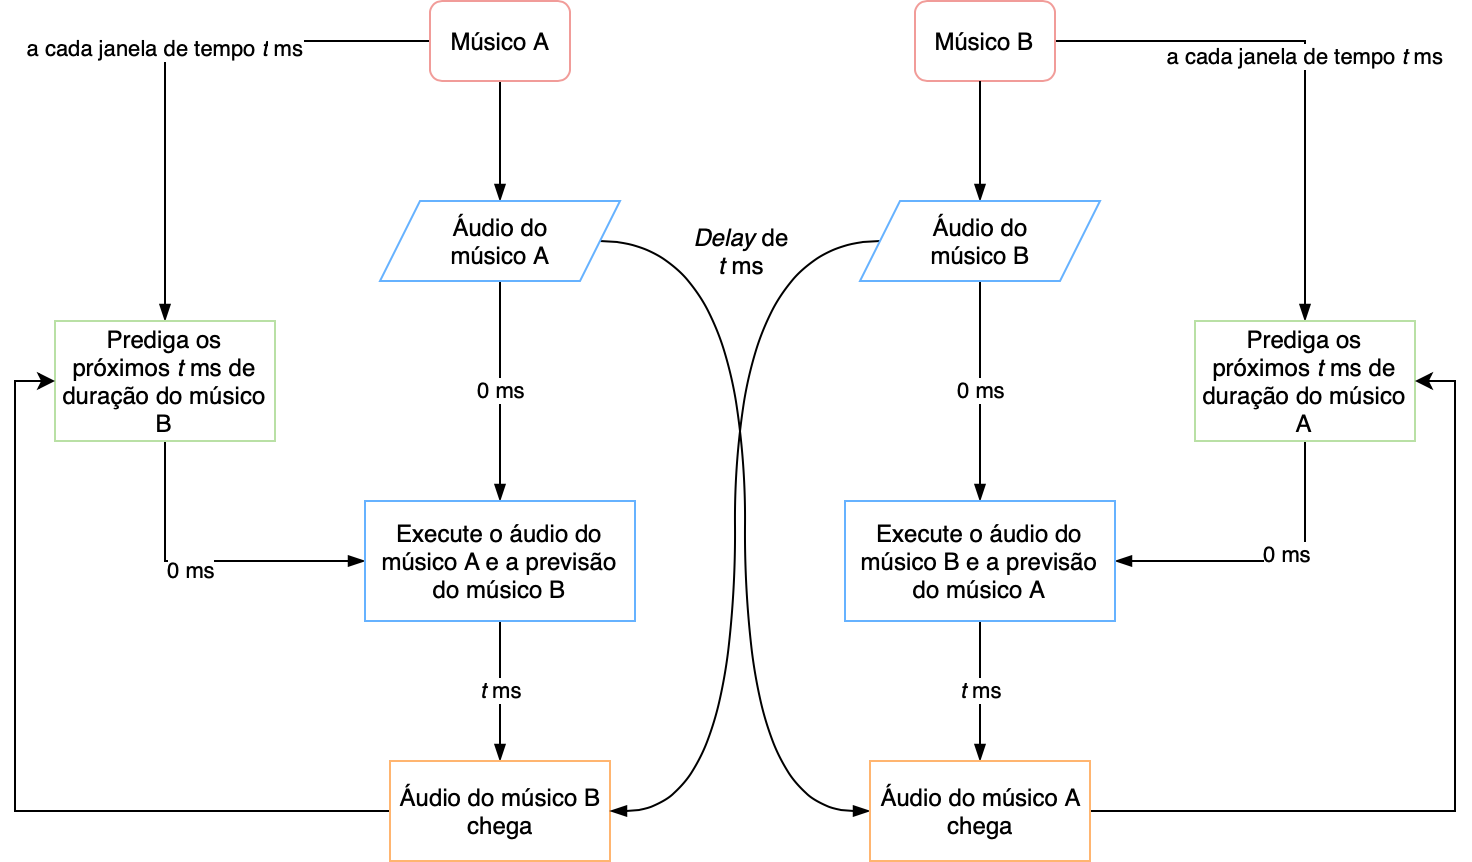
\includegraphics[width=1\textwidth]{images/rollback-music.png}
\caption{Diagrama demonstrando a adaptação do algoritmo de previsão no lado do cliente aplicado para \textit{streaming} colaborativo de música \textit{online}. Na imagem, "X" representa a duração da janela de previsão, medido em milissegundos.}
\label{fig:rollback_music_diagram}
\end{figure}

Em Bernier, a janela de tempo de cada conjunto de previsões é definida de acordo com o FPS e a velocidade de conexão entre os participantes. Na adaptação musical, além do tempo de ida e volta dos pacotes entre os participantes (\textit{ping}), propomos a utilização de outros parâmetros para a decisão dessa janela, como o BPM (batimentos da música) ou valores arbitrários. A escolha dessa janela é fundamental - durações muito longas possuem muita informação, porém, são mais difíceis de processar; e o inverso ocorre para janelas muito curtas.

Propomos, portanto, dois modelos preditivos para música, dividido em dois ciclos de pesquisa. No (CITAR CAPITULO), utilizamos a arquitetura de aprendizagem de máquina em camadas LSTM (\textit{Long short-term memory)} \cite{lstm} para gerar sequências de sinais digitais. Já em (CITAR CAPITULO), no segundo ciclo, usamos o algoritmo DTW (\textit{Dynamic Time Warping}) \cite{dtw} para identificar janelas semelhantes em uma base de dados e, a partir dessa informação, reproduzir a próxima janela de áudio, também armazenada na mesma base de dados.


% Ao observar o contexto de videogames, encontramos requisitos de latência similares. Gêneros que utilizam reações como mecânica de jogabilidade, como luta e FPS (\textit{first-person shooter}), para oferecerem aos jogadores uma experiência fluida, necessitam de latências máximas de até 100 ms \cite{pubnub}. O algoritmo mais popular e efetivo para solucionar esse problema, \textit{client-side prediction} \cite{client-side-prediction}, baseia-se em prever os próximos \textit{inputs} imediatos dos jogadores e agindo antes mesmo que os dados de seu oponente sejam transmitidos; desta forma, removendo a necessidade inicial de espera. Uma vez que os \textit{inputs} são recebidos, estes são comparados com a previsão realizada e, caso sejam incongruentes entre si, o jogo é retornado ao estado anterior do momento da previsão inicial.

% Por possuir requisitos semelhantes de baixa latência, a mesma implementação baseada em previsões tem o potencial de resolver o problema descrito anteriormente para ambientes musicais colaborativos \textit{online}. Caso seja possível prever os próximos sinais digitais produzidos pelos artistas remotos, não haveria necessidade de espera e, portanto, a latência de rede tornaria-se irrelevante.

% Evidentemente, as diferenças entre os contextos de \textit{videogames} e práticas musicais não são negligenciáveis. Ao contrário dos jogos, por apresentar uma linearidade no tempo, não é possível retornar ao último momento da música anterior à previsão imediata sem atrapalhar a performance dos artistas. Além disso, a natureza discreta dos \textit{inputs} dos \textit{videogames} e a quantidade bruta de dados produzida é ínfima em comparação à áudios digitais - estima-se que os jogadores profissionais de \textit{Super Smash Bros. Melee} mais técnicos produzem em média 6 \textit{inputs} por segundo \cite{melee_inputs_per_second}; uma transmissão de áudio com \textit{sample rate} de 44,1 khz produz, por definição, 44.100 diferentes valores no mesmo espaço de tempo \cite{jukebox_dimension}. Portanto, a aplicação do algoritmo de \textit{client-side prediction} para transmissão de música \textit{online} não é trivial, e a necessidade que o modelo preditivo seja o mais acurado possível é ainda mais importante.